\documentclass{article}

\usepackage{amsmath}
\usepackage{amssymb}
\usepackage{amsfonts}
\usepackage{mathtools}

\usepackage[thmmarks, amsmath]{ntheorem}

\usepackage{graphicx}
\usepackage{float}
\usepackage{tikz-cd}
\usepackage{adjustbox}

\usepackage{diffcoeff}
\diffdef{}{op-symbol=\mathrm{d},op-order-sep=0mu}

\usepackage{cancel}
\usepackage{interval}

\usepackage{array}

\usepackage{enumitem}

\setlist[enumerate,1]{label=(\alph*)}

\title{Algebraic Topology Homework 4}
\author{Duarte Maia}
%\date{}

\theoremstyle{plain}
\theorembodyfont{\upshape}
\theoremseparator{.}
\newtheorem{theorem}{Theorem}
\newtheorem{prop}{Prop}
\renewtheorem*{prop*}{Prop}
\newtheorem{lemma}{Lemma}
\newtheorem*{ex}{Exercise}

\theoremstyle{nonumberplain}
\theoremheaderfont{\itshape}
\theorembodyfont{\upshape}
\theoremseparator{:}
\theoremsymbol{\ensuremath{\blacksquare}}
\newtheorem{proof}{Proof}
\newtheorem{sol}{Solution}

\theoremsymbol{\text{\textit{(End proof of lemma)}}}
\newtheorem{lemmaproof}{Proof of lemma}

\newcommand{\R}{\mathbb{R}}
\newcommand{\C}{\mathbb{C}}
\newcommand{\Z}{\mathbb{Z}}
\newcommand{\Q}{\mathbb{Q}}

\newcommand{\RP}{\mathbb{RP}}

\newcommand{\kk}{\Bbbk}

\newcommand{\PP}{\mathbb{P}}
\newcommand{\FF}{\mathcal{F}}

\newcommand{\I}{\mathrm{i}}
\newcommand{\e}{\mathrm{e}}

\newcommand{\id}{\mathrm{id}}
\newcommand{\GL}{\mathrm{GL}}

\newcommand{\conj}[1]{\overline{#1}}
\newcommand{\close}[1]{\overline{#1}}

\DeclareMathOperator{\inte}{int}
\DeclareMathOperator{\codim}{codim}
\DeclareMathOperator{\trace}{tr}
\newcommand{\grad}{\nabla}


\DeclareMathOperator{\spec}{spec}

\DeclarePairedDelimiter{\abs}{\lvert}{\rvert}
\DeclarePairedDelimiter{\norm}{\lvert}{\rvert}
\DeclarePairedDelimiter{\Norm}{\lVert}{\rVert}
\DeclarePairedDelimiter{\braket}{\langle}{\rangle}


\begin{document}
\maketitle

\begin{ex}[2.2:7]
Let $f \in \GL(\R^n)$, $n \geq 1$. Show that the induced automorphism on $H_n(\R^n, \R^n \setminus 0) \cong \Z$ is plus or minus the identity, depending on whether $f$ preserves or reverses orientation.
\end{ex}

\begin{sol}
It is a known fact (I've done it for algebra homework a few weeks back and don't feel like doing it again) that $\GL(\R^n)$ has exactly two path-connected components, classified by the sign of the determinant. Thus, $f$ is either homotopic to $I$ or $J$, where $J(x_1, \dots, x_n) = (-x_1, x_2, \dots, x_n)$. Obviously $I$ induces the identity in homology, so it suffices to show that $J$ induces minus the identity in homology.

To this effect, we use the fact that the following diagram commutes, where $R \colon S^n \to S^n$ is reflection on the first component.
\begin{figure}[H]
\centering
\begin{tikzcd}
{\R^n, \R^n \setminus 0} \arrow[d, "J"] \arrow[r, "\cong", phantom] & {D^n, D^n \setminus 0} \arrow[d, "J"] & {D^n, S^{n-1}} \arrow[l, "i"'] \arrow[r, "\pi"] \arrow[d, "J"] & {S^n, *} \arrow[d, "R"] \\
{\R^n, \R^n \setminus 0} \arrow[r, "\cong", phantom]                & {D^n, D^n \setminus 0}                & {D^n, S^{n-1}} \arrow[l, "i"'] \arrow[r, "\pi"]                & {S^n, *}               
\end{tikzcd}
\end{figure}

Applying the homology functor to this diagram, all horizontal maps become isomorphisms (by excision and other stuff), and $R$ becomes minus the identity (this has been established when we've talked about degree). Since $-1$ commutes with all other isomorphisms, all maps $J$ induce $-1$ in homology.
\end{sol}

\begin{ex}[2.2:18]
Let $(X,A)$ be a CW pair. Show that there is a relative cellular chain complex formed by $H_i(X^i, X^{i-1} \cup A^i)$ with homology groups isomorphic to $H_n(X,A)$.
\end{ex}

\begin{sol}
First, consider the relative long exact sequence applied to the triple $(X^i, X^{i-1} \cup A^i, A^i)$. We obtain
\begin{multline}
\cdots \to H_{k+1}(X^i, X^{i-1} \cup A^i) \to H_k(X^{i-1} \cup A^i, A^i) \\\to H_k(X^i, A^i) \to H_{k}(X^i, X^{i-1} \cup A^i) \to H_{k-1}(X^{i-1} \cup A^i, A^i) \to \cdots
\end{multline}

Now, since CW pairs are good pairs, the first term is isomorphic to $\tilde H_{k+1}(X^i / (X^{i-1} \cup A^i))$, and this space is homeomorphic to a wedge of $i$-spheres, so this homology group is null whenever $k \neq i-1$. Likewise, $H_k(X^i, X^{i-1} \cup A^i) = 0$ whenever $k \neq i$. Thus, the standard argument used in cellular homology (induction $+$ weak topology to reduce to finite case), together with some excision to show $H_k(X^{i-1} \cup A^i, A^i) \cong H_k(X^{i-1}, A^{i-1})$ (apply excision to remove the center of each $i$-cell of $A$ and then retract by deformation to $X^{i-1}$), shows that $H_k(X,A) \cong H_k(X^{k+1}, A^{k+1})$ Moreover, for $i = k+1$ the LES gives us
\begin{equation}\label{eq:les1}
\begin{multlined}
H_{k+1}(X^{k+1}, X^{k} \cup A^{k+1}) \xrightarrow{F} H_{k}(X^{k} \cup A^{k+1}, A^{k+1}) \\\to H_{k}(X^{k+1}, A^{k+1}) \to H_{k}(X^{k+1}, X^{k} \cup A^{k+1})
\end{multlined}
\end{equation}

Now, notice that $H_k(X^{k+1}, X^k \cup A^{k+1}) = 0$ because by excision this coincides with $H_k(X^{k+1} / (X^k \cup A^{k+1}))$ which is a wedge of $k+1$-balls. Hence,
\begin{equation}
H_k(X,A) \cong H_k(X^{k+1}, A^{k+1}) \cong \frac{H_k(X^k \cup A^{k+1}, A^{k+1})}{\text{something}} \cong \frac{H_k(X^k, A^{k})}{\text{something}}.
\end{equation}

Now, for $i = k$ we get
\begin{equation}
\begin{multlined}
H_{k}(X^{k-1} \cup A^{k}, A^{k}) \to H_{k}(X^{k}, A^{k})\\\to H_{k}(X^{k}, X^{k-1} \cup A^{k}) \xrightarrow{F} H_{k-1}(X^{k-1} \cup A^k, A^k)
\end{multlined}
\end{equation}
and the first term is null for the same reason, hence $H_k(X^k, A^k)$ can be seen as a subgroup of $H_k(X^k, X^{k-1} \cup A^k)$, namely the kernel of the map $F$ above.

Ahhh, this is getting messy, but I think I know what diagram I need to draw now. Here it is:
\begin{figure}[H]
\centering
\adjustbox{scale=0.7, center}{
\begin{tikzcd}
             &                            &                                                          & 0 \arrow[rd]                                                 &                                        &                                                     &                                          \\
             &                            &                                                          & {H_{k-1}(X^{k-1} \cup A^k, A^k)} \arrow[r, "\cong", phantom] & {H_{k-1}(X^{k-1}, A^{k-1})} \arrow[rd] &                                                     &                                          \\
             &                            & {H_k(X^k, X^{k-1} \cup A^k)} \arrow[ru,"F"] \arrow[rrr, "D"] &                                                              &                                        & {H_{k-1}(X^{k-1}, X^{k-2} \cup A^{k-1})} \arrow[rd] &                                          \\
             & {H_k(X^k, A^k)} \arrow[ru] &                                                          &                                                              &                                        &                                                     & {H_{k-2}(X^{k-2} \cup A^{k-1}, A^{k-1})} \\
0 \arrow[ru] &                            &                                                          &                                                              &                                        &                                                     &                                         
\end{tikzcd}
}
\end{figure}

Alright so, the map $D$ above is the chain map I'm looking for. $D \circ D = 0$ with the same proof for cellular homology (somewhere along the way you do two maps in an exact sequence in a row). Now, note that $D$ is a composition of three maps, all of which except $F$ are injective, so $\ker D = \ker F = H_k(X^k, A^k) \cong H_k(X^k \cup A^{k+1}, A^{k+1})$. Moreover, under these identifications, the image of $D$ coincides with the image of $F$ inside this group. Thus, the homology of the chain complex with $D$ is identified with the cokernel of $F$, and using \eqref{eq:les1} this cokernel coincides with the relative homology $H_k(X,A)$, so we're done.1\
\end{sol}

\begin{ex}[2.2:29]
Compute the homology groups of $X$ using the Mayer-Vietoris sequence for the given decomposition of $X$ into two copies of $R$. Compute also the relative groups $H_i(R,M)$ with $M = M_g$.
\end{ex}

\begin{sol}
We begin by noting that $(X,M)$ is a good pair, because $(R, M)$ is a good pair. Let $U$ be a neighborhood of $M$ in $X$ which deformation retracts to $M$. Now, let $A = R \cup U$ and $B = R \cup U$, where each of them refers to a distinct copy of $R \subseteq X$. I know the notation is silly, but I'm sure the reader will understand what I mean.

Now, $X = A \cup B$ and both $A$ and $B$ are open, so the Mayer-Vietoris sequence applies
\begin{equation}
\cdots \to H_n(A \cap B) \to H_n(A) \oplus H_n(B) \to H_n(X) \to H_{n-1}(A \cap B) \to \cdots
\end{equation}

Now, note that $A$ and $B$ are both homotopically equivalent to $R$, which retracts by deformation to a wedge of $g$ circles,, and $A \cap B$ is homotopically equivalent to $M$. This means that we know pretty well the homologies of $A$, $B$, and $A \cap B$:
\begin{equation}
\begin{aligned}
H_n(A) \cong H_n(B) &\cong \begin{cases}
0 & \text{if $n > 1$,}\\
\Z^g & \text{if $n = 1$,}\\
\Z & \text{if $n = 0$,}
\end{cases}\\
H_n(A \cap B) &\cong \begin{cases}
0 & \text{if $n > 2$,}\\
\Z & \text{if $n = 2$,}\\
\Z^{2g} & \text{if $n = 1$,}\\
\Z & \text{if $n = 0$,}
\end{cases}
\end{aligned}
\end{equation}
where the computation of $H_n(A \cap B) \cong H_n(M)$ is done in example 2.36 of Hatcher.

With this data, we see that the Mayer-Vietoris sequence looks like
\begin{equation}
\begin{aligned}
\cdots &\to 0 \to 0 \oplus 0 \to H_3(X) \to \\
&\to \Z \to 0 \oplus 0 \to H_2(X) \to\\
&\to \Z^{2g} \to \Z^{g} \oplus \Z^{g} \to H_1(X) \to\\
&\to \Z \to \Z \oplus \Z \to H_0(X) \to 0.
\end{aligned}
\end{equation}

We see immediately that $H_3(X) \cong \Z$. Moreover, $H_2(X)$ is identified with a subgroup of $\Z^{2g}$, namely the kernel of the map $\Z^{2g} \to \Z^g \oplus \Z^g$, so we had better find out what this map is.

This map has two components, each of which is induced by the inclusion $M \hookrightarrow R$. We claim that this map is a projection on $g$ components. Indeed, the following picture shows the generators of $M$ and $R$ (these are known), and it is obvious that the ones denoted in red are killed off by the inclusion (they become contractible), while the ones denoted in blue are preserved.
\begin{figure}[H]
\centering
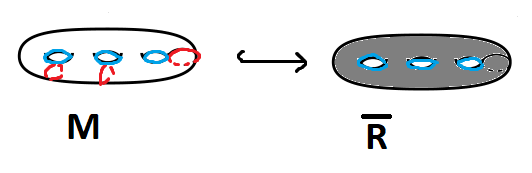
\includegraphics[width=\linewidth]{mt3_fix}
\end{figure}

Now, note that this is the same projection in both components, so the map $p \colon \Z^{2g} \to \Z^g \oplus \Z^g$ is given by $p(x_1, \dots, x_{2g}) = (x_1, \dots, x_g, x_1, \dots, x_g)$. Thus, its image is the diagonal $D \subseteq \Z^g \oplus \Z^g$ and its kernel is $0 \times \Z^g$ (hence $H_2(X) \cong \Z^g$).

We then have the following exact sequence.
\begin{equation}
\Z^{2g} \xrightarrow{p} \Z^g \oplus \Z^g \xrightarrow{q} H_1(X) \to \Z \to \Z \oplus \Z \to (H_0(X) \cong \Z) \to 0,
\end{equation}
where $H_0(X)$ is isomorphic to $\Z$ because $X$ is path connected and nonempty.

Now, if we can show that the map $\Z \to \Z \oplus \Z$ is null, we have the exercise done, because then $H_1$ is isomorphic to $(\Z^g \oplus \Z^g)/D \cong \Z^g$. We could do this directly, but instead we will use the following trick: use Mayer-Vietoris for reduced homology instead! If we do this, the zeroth homology of $A \cap B$ becomes null, and we instead have the exact sequence
\begin{equation}
\xrightarrow{q} \Z^g \oplus \Z^g \to H_1(X) \to 0,
\end{equation}
which proves that $H_1 \cong (\Z^g \oplus \Z^g)/D \cong \Z^{g}$. This completes the computation of the homology of $X$:
\begin{equation}
H_n(X) \cong \begin{cases}
0 & \text{if $n > 3$,}\\
\Z & \text{if $n = 3$,}\\
\Z^{g} & \text{if $n = 2$,}\\
\Z^{g} & \text{if $n = 1$,}\\
\Z & \text{if $n = 0$.}
\end{cases}
\end{equation}

\medskip

Now, to compute the relative groups, we use the long exact sequence for the pair $(R,M)$. It looks very similar, because where before we had $H_n(A \cap B)$ we now have the isomorphic $H_n(M)$, and where we had $H_n(A) \oplus H_n(B) \cong H_n(R) \oplus H_n(R)$ we now have just $H_n(R)$.
\begin{equation}
\begin{aligned}
\cdots &\to 0 \to 0 \to H_3(R,M) \to \\
&\to \Z \to 0 \to H_2(R,M) \to\\
&\to \Z^{2g} \to \Z^{g} \to H_1(R,M) \to\\
&\to \Z \to \Z \to H_0(R,M) \to 0.
\end{aligned}
\end{equation}

Now, the same arguments that before showed that certain maps were null (and the thing that was the diagonal is now just the projection in $g$ components) still hold, and therefore we have, by exactly the same reasons,
\begin{equation}
H_n(R,M) \cong \begin{cases}
0 & \text{if $n > 3$,}\\
\Z & \text{if $n = 3$,}\\
\Z^{g} & \text{if $n = 2$,}\\
0 & \text{if $n = 1$,}\\
0 & \text{if $n = 0$.}
\end{cases}
\end{equation}
\end{sol}

\begin{ex}[2.2:33]
Suppose $X$ is the union of open sets $A_1, \dots, A_n$ such that all finite intersections have trivial reduced homology groups or are empty. Show that $\tilde H_i(X) = 0$ for $i \geq n-1$, and that this inequality is sharp.
\end{ex}

\begin{sol}
Induction on $n$. For $n = 1$ this is obvious by hypothesis, so now we assume that it is true for some $n$ and prove it for $n+1$. As such, let $X = Y \cup A_{n+1}$, with $Y = A_1 \cup \dots \cup A_n$. We now apply reduced Mayer-Vietoris to get the exact sequence
\begin{equation}\label{eq:mv}
\cdots \to \tilde H_i(Y \cap A_{n+1}) \to \tilde H_i(Y) \oplus \tilde H_i(A_{n+1}) \to \tilde H_i(X) \to \tilde H_{i-1}(Y \cap A_{n+1}) \to \cdots
\end{equation}

Note that by the induction hypothesis, $Y$ has null reduced homology from degree $n-1$ onwards. This also applies for $Y \cap A_{n+1} = \bigcup_{j=1}^n (A_j \cap A_{n+1})$. Thus, \eqref{eq:mv} tells us that, whenever $i-1 \geq n-1$, i.e. whenever $i \geq n$, we have $\tilde H_i(X) \cong \tilde H_i(Y) \oplus \tilde H_i(A_{n+1}) \cong 0 \oplus 0$ by the IH. This completes the proof.

To get that the inequality is sharp, let $X = \partial \Delta^{n-1}$, and $A_i$ be a small neighborhood of the $i$-th face of $X$, for $i = 0, \dots, n-1$. Thus, these $A_i$ satisfy the hypotheses, as the intersection of $k$ of them will be a small neighborhood of an $n-2-k$-simplex, which is contractible and hence has null homologies. However, $X$ itself has non-null $n-2$-th homology, which shows that the inequality cannot go lower than $n-1$.
\end{sol}

\begin{ex}[2.2:35]
Show that if $X$ is a finite simplicial complex whose first homology has nontrivial torsion, then there is no embedding of $X$ in $\R^3$ such that some neighborhood of $X$ retracts by deformation onto $X$ and is homeomorphic to the mapping cylinder of some map from a closed orientable surface $S$ to $X$.
\end{ex}

\begin{sol}
Let $A$ be the interior of this neighborhood (which is homeomorphic to the mapping cylinder with the top removed), and let $B = \R^3 \setminus X$. Since $A \cup B = \R^3$ which has null homology, the Mayer-Vietoris sequence simply gives us that $H_1(A \cap B) \cong H_1(A) \oplus H_1(B)$. Now, $A \cap B$ is homeomorphic to the mapping cylinder of a map from $S$ to $X$, with the bottom and top removed, i.e. $S \times \left]0,1\right[ \simeq S$, and by the classification of closed orientable surfaces we know that $H_1(A \cap B) \cong H_1(S)$ has no torsion. This means that $H_1(A)$ cannot have torsion, and since $A \simeq X$ we get that $H_1(X)$ cannot have torsion either, which completes the proof.
\end{sol}

\begin{ex}[2.C:4]
Show that the Euler characteristic of the set of fixed points $Y$ of a simplicial homeomorphism $f \colon X \to X$ is the Lefschetz number of $f$.
\end{ex}

\begin{sol}
First, let $X'$ be the (once) barycentric subdivision of $X$. Then, we claim that $Y$ is a subcomplex of $X'$. Indeed, to this effect, it suffices to prove the following lemma: given a linear endomorphism of the $N$-simplex, the set of fixed points of this endomorphism is a subcomplex of the barycentric subdivision of the simplex. Once this lemma is proven, we perform the following procedure on $X$. We look at each simplex, and see if it is taken to itself. If not, then its interior has no fixed points. Otherwise, $f$ restricts to an automorphism of this simplex and thus the lemma applies.

To show the lemma, we first note that we can characterize the set of fixed points very well. Since a linear endomorphism of the $N$-simplex $\Delta$ is determined by a permutation of the vertices, and therefore of the barycentric coordinates, we can characterize it as follows. Decompose this permutation into its cycles. Then, for each cycle, all the coordinates must coincide, and if this holds for all cycles of the permutation then we have a fixed point. Thus, the set of fixed points is determined by a collection of equations of the form $x_i = x_j$. The set of solutions to any such equation is (by construction and induction) a subcomplex of $\Delta'$, and finally, intersections of subcomplexes are themselves subcomplexes.

Now that the lemma is proven, we may assume that $Y$ is a subcomplex of $X$ without loss of generality. Now, we apply the definition of $\tau(f)$:
\begin{equation}
\tau(f) = \sum (-1)^i \trace f_i,
\end{equation}
and we apply the formula $\trace f_k = \trace f_{\sharp Z k} - \trace f_{\sharp B k}$, where $f_{\sharp Z k}$ is the map induced by $f$ on $Z_k$ and likewise for $f_{\sharp B k}$ (and soon, for $f_{\sharp C k}$).

Moreover, we also have the formula $\trace f_{\sharp Z k} + \trace f_{\sharp B (k-1)} = \trace f_{\sharp C k}$, so applying the same tricks we use in the proof that the Euler number of a space equals the thing with the cells of each dimension, we obtain
\begin{equation}
\tau(f) = \sum (-1)^i \trace f_{\sharp C k}.
\end{equation}

Now, note that since $f$ is a simplicial homeomorphism, its matricial representation in $C_k$ is a matrix with just a bunch of ones, exactly one per column. As such, the trace counts exactly how many ones there are in the diagonal, that is, how many simplices of dimension $k$ are kept fixed by $f$. In other words, \emph{the number of simplices of dimension $k$ in $Y$}.

With these last few words we can just apply the definition of Euler characteristic for a CW/$\Delta$ complex, and we are done.
\end{sol}

\end{document}